\documentclass[12pt,ngerman,twopage]{scrartcl}
\usepackage[utf8]{inputenc}
\usepackage[T1]{fontenc}
\usepackage{ngerman}
\usepackage[hyphens]{url}
\usepackage[linkcolor=blue,urlcolor=red]{hyperref}
\usepackage{graphicx}
\usepackage{fmtcount}
\newcommand{\datum}{19.10.2013}
\title{UEFI\\{\large Die neue Art zu booten}}
\date{\datum}
\author{Oliver Schmidt}
\begin{document}
\maketitle
\tableofcontents
\clearpage

\twocolumn
\section{Einleitung}
Der Personal Computer hat gegenüber vielen anderen Computersystemen (wie z.B. modernen Smartphones mit ARM Architektur) die Besonderheit, dass Kernbestandteile des Hardwaresystems wie etwa die CPU oder Erweiterungskarten und auch die Softwarekomponenten wie das Betriebssystem einfach austauschbar sind. Damit dies möglich ist und Software- und Hardwarekomponenten auf allen Systemen funktionsfähig sind, wird eine \textit{Firmware} benötigt, die standardisierte Schnittstellen zwischen den Hardware- und Softwarekomponenten bereitstellt. Diese Firmware ist die erste Software, die nach dem Start des Systems ausgeführt wird und ebnet den Weg für nicht hardwarespezifische Software, indem es externe (nicht zum Chipsatz auf dem Motherboard gehörende) Hardware erkennt, initialisiert, über Schnittstellen  zugreifbar macht und zuletzt dann das Betriebssystem startet.
\section{Basic Input Output System (BIOS)}
Jeder PC Nutzer kennt sie, die kryptischen Meldungen, die nach dem Einschalten des PCs zu sehen sind, bevor sich dann das eigentliche Betriebssystem meldet. Mittlerweile sind diese allerdings oft hinter einem versteckt und der Nutzer sieht nur noch ein verpixeltes Herstellerlogo. Diese Meldungen stammen vom \textit{BIOS}, dem \textit{Basic Input Output System}.
\subsection{IBM PC}
Dieses BIOS wurde im Jahr 1981 mit dem IBM PC eingeführt. Dieses Gerät war ein kleiner Heimcomputer, auf dem verschiedene Betriebssysteme lauffähig waren. Zumeist wurde das Betriebssystem MS-DOS von Microsoft verwendet, welches jedoch auch auf anderen Computern lauffähig war. Somit war der größte Teil der Software nicht ausschließlich auf die IBM Hardware zugeschnitten, die einzige speziell auf die Hardware zugeschnittene Software war die Firmware des Computers, das \textit{PC BIOS}.
Der Erfolg des IBM PCs führte zum Entstehen eines großen Marktes an IBM PC kompatibler Hardware als auch nur auf IBM PCs lauffähiger Software. Dieser große Markt veranlasste auch andere Hersteller wie etwa Compaq, Computer zu bauen, die ebenfalls diese Produkte nutzen konnten. Dies war nur möglich, wenn der Hardwarespezifische Teil, in diesem Fall das PC BIOS, auch in diesen Geräten vorhanden war. Aus urheberrechtlichen Gründen durfte das PC BIOS jedoch nicht einfach kopiert werden, sondern musste durch reverse engineering nachgebaut werden. Schon wenige Jahre nach dem erscheinen des Original IBM PCs gab es somit eine Vielzahl von Klonen, die allesamt unabhängig und ohne Zusammenarbeit mit IBM entstanden. Diese „IBM-PC kompatiblen Computer“ traten ihren Siegeszug an, verdrängten Konkurrenzsysteme wie Atari und bis heute sind nahezu alle verkauften Heimcomputer und Notebooks kompatibel zum IBM PC, können also so genutzt werden wie damals der IBM PC mit MS-DOS.
\subsection{Aufgaben}
\subsubsection{Der Bootprozess}
Das BIOS ist die erste Software, die nach dem Start des PCs ausgeführt wird. Zuallererst wird der \textit{Power On Self Test (POST)} durchgeführt. Dabei erkennt und initialisiert das BIOS die Systembestandteile wie CPU, RAM, diverse Controller (DMA, interrupt Controller), Chipsatz und angeschlossene Geräte. Wenn das BIOS bootfähige Speichergeräte findet, lädt es die im \textit{Master Boot Record (MBR)} befindliche Bootloader Software und übergibt dieser die Kontrolle über den PC. Der Bootloader lädt dann den Kernel eines Betriebssystems.
\subsubsection{weitere Aufgaben}
Das BIOS stellt grundlegende Dienste für das Betriebssystem in einer standardisierten Form zur Verfügung. MS-DOS für den PC etwa benutzte das BIOS als Hardwareabstraktionsschicht und griff zur Kommunikation mit bestimmten Systemkomponenten wie Speicher-, Eingabe- oder Ausgabegeräten auf dessen Funktionen zurück.

Moderne BIOS Software besitzt oftmals eine textbasierte Konfigurationsoberfläche, in der verschiedene Systemeinstellungen verändert werden können. So kann zum Beispiel das primäre Bootgerät festgelegt werden oder die Spannung bzw. die Taktfrequenz der CPU verändert werden. Beim originalen PC BIOS konnten Einstellungen über Jumper gesetzt werden.
%ACPI?
\subsection{Probleme}
Um die Kompatibilität zum originalen PC BIOS und MS DOS zu bewahren, müssen auch 32-bit Prozessoren einen Intel 8086 16-bit Prozessor besitzen wie auch der IBM PC ihn besaß. Dieser existiert zwar mittlerweile nur noch virtuell und wird durch durch Emulation realisiert, stellt aber trotzdem noch eine Altlast dar.

Das BIOS läuft auch auf moderner 32- oder 64-bit Hardware immer noch im 16-bit real mode und kann damit selbst nur 1 MiB Speicher adressieren. Damit ist der Hardwarezugriff über das BIOS für moderne multitaskingfähige 32- oder 64-bit Betriebssystemkernel wie Windows NT oder Linux zu langsam und ineffizient, weshalb sie die Hardwarezugriffe selbst koordinieren. Dazu greifen sie direkt über eigene Treibersoftware auf die Hardwarekomponenten zu. Ein weiterer Vorteil der betriebssystemeigenen Treiber ist, dass durch Betriebssystemupdates Unterstützung für neue Hardware hinzugefügt werden kann, ohne dass die Firmware des Computers geändert werden muss.

Im boot code Bereich des \textit{MBR} können nur bis zu 440byte große Programme abgelegt werden. Heutige komplexere Bootloader passen dort nicht mehr hinein, sondern es wird nur noch Code vom BIOS gestartet (Stage 1), welcher den Bootloader aus einem Dateisystem liest und ausführt (Stage 2). Auch kann es nur einen Bootloader geben, der nach dem Start vom BIOS gestartet wird, weshalb für Multi-Boot Systeme mit mehreren Betriebssystemen ein Multi-Boot fähigen Bootloader wie etwa GRUB benötigt wird, welcher dann eine Auswahlmöglichkeit zwischen den zu startenden Betriebssystemen ermöglicht und dann den Kernel oder einen anderen Bootloader nachlädt (chainloading).

Somit wird das BIOS nur noch zum Starten des Betriebssystems bzw. des Bootloaders, welcher dann das Betriebssystem lädt, benötigt, während andere Fähigkeiten mittlerweile überflüssig geworden sind oder nur noch überflüssige Altlasten darstellen.
\section{Unified Extensible Firmware Interface (UEFI)}
Und genau der Bootvorgang ist das Hauptproblem, für das \textit{UEFI} gedacht ist. Für leistungsfähigere System wie Serversysteme wurden die Einschränkungen des BIOS sehr schnell zu einem Problem, deshalb begann Intel Jahr 1998, mit der „Intel Boot Initiative“ eine Alternative zu entwickeln. 2005 wurde dann das mittlerweile zu \textit{EFI (Extensible Firmware Interface)} umbenannte Ergebnis als EFI 1.10 veröffentlicht und an das neu gegründete Unified EFI Forum\footnote{\url{http://uefi.org}} übergeben, welches den Standard seitdem als \textit{UEFI (Unified Extensible Firmware Interface)} weiterentwickelt. Im Gegensatz zum BIOS ist UEFI somit kein Stück geschlossene Software, das durch reverse-engineering nachgebaut wurde, sondern eine offene Spezifikation, die von einem Standardisierungsgremium entwickelt wird und an der mehrere Firmen mitwirken.
\subsection{Verbesserungen}
Die UEFI Firmware kann entweder 32- oder 64-bit Software (je nach Prozessor) sein und damit auf sämtlichen vom Prozessor adressierbaren Speicher zugreifen, somit ist das 1 MiB Limit des BIOS hinfällig.
UEFI ist auch prozessorunabhängig designt und prinzipiell auf allen little-endian Architekturen lauffähig.  UEFI 2.3 läuft derzeit auf den Prozessorarchitekturen x86, x86\_64, ARM und Itanium.

UEFI benutzt das neue \textit{GPT (GUID Partition Table)} Schema und kann damit auch, anders als BIOS Versionen, die GPT unterstützen, auch von Festplaten größer als 2 TiB booten. Es wird auch noch das alte MBR Schema unterstützt, es ist aber nur zur Abwärtskompatibilität gedacht.

Selbst wenn doch noch das veraltete MBR Partitionierungsschema verwendet wird, existiert das Problem des für moderne Bootloader nicht mehr ausreichenden Speicherplatzes im boot code Bereich des MBR nicht mehr, da UEFI Dateisysteme lesen kann: Laut UEFI Standard müssen die Dateisysteme FAT12, FAT16 und VFAT (FAT32) unterstützt werden. Diese werden dann für eine EFI Systempartition verwendet, auf der mehrere Bootloader als ausführbare Dateien liegen. Damit ist auch das Multiboot Problem gelöst, da nun jedes Betriebssystem seinen eigenen Bootloader installieren kann und das UEFI eine Auswahlmöglichkeit bietet.
\subsection{Aufbau}
\addtocounter{footnote}{1}
\footnotetext[\value{footnote}]{Grafik von Msikma unter \href{CC_BY-SA}{https://creativecommons.org/licenses/by-sa/2.5/deed.en}}
\begin{figure}[h]
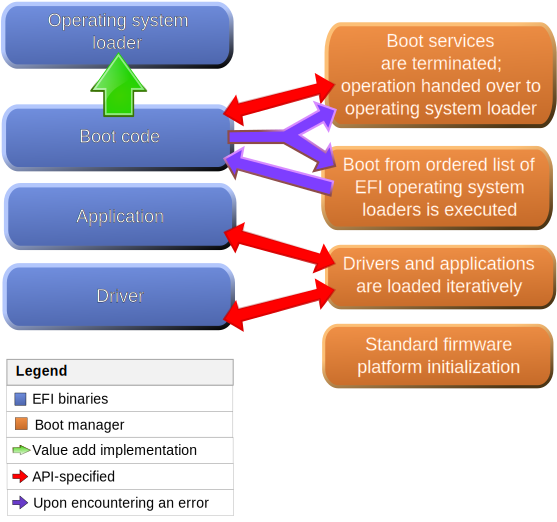
\includegraphics[width=\linewidth]{EFI-bootprocess}
\caption{Der UEFI Bootprozess$^{\decimal{footnote}}$}

\end{figure}
Große Teile von UEFI wurden von Intel als „TianoCore“\footnote{
\url{http://sourceforge.net/apps/mediawiki/tianocore/index.php?title=Welcome\_to\_TianoCore}} unter einer BSD Lizenz freigegeben. Somit besteht die Referenzimplementierung von UEFI zu einem Großteil aus OpenSource Software. Diese Referenzimplementierung wird meist zu großen Teilen auch in den UEFI Implementierungen der einzelnen Hersteller verwendet, allerdings gibt es auch vollständig proprietäre Implementierungen. Dies alles setzt aber meist auf proprietärem, hardwarespezifischem Initialiasierungscode auf, der vergleichbar mit der POST Phase des Bios ist. Danach wird jedoch das UEFI System von einem Speicherchip, von der Festplatte oder sogar aus dem Netzwerk als schon fast eine Art Betriebssystem geladen.

\subsubsection{Features}
UEFI kennt 2 Klassen sogenannter Services: Boot services und runtime services. Boot services werden nur beim Start des Computer ausgeführt und enden, sobald das Betriebssystem die Kontrolle übernimmt, während runtime services auch nach dem Start des Betriebssystems weiterlaufen. Diese können mit dem Betriebssystem interagieren, etwa zur Zeiteinstellung oder um Fehlermeldungen nach einem Systemcrash in das UEFI Log zu schreiben.
UEFI ist modular aufgebaut, kann also durch weitere Komponenten erweitert werden, diese müssen aber ein bestimmtes Protokoll zur Kommunikation mit UEFI unterstützen. Dieses Protokoll ist im UEFI Standard festgelegt.

Solche Erweiterungen sind etwa Gerätetreiber, die in prozessorunabhängigem EFI Byte Code geschrieben sind. Dieser Bytecode wird dann von einem Interpreter, der im UEFI integriert ist, interpretiert und ausgeführt. Der Vorteil für Gerätehersteller ist, dass diese zumindest die UEFI Treiber nur einmal entwickeln müssen und sie dann architekturunabhängig einsetzen können. Diese können jedoch nicht vom Betriebssystem genutzt werden, das Betriebssystem kann nur mit einigen wenigen prozessorspezifischen Treibern interagieren, die gerade den Vorteil der Plattformunabhängigkeit nicht besitzen.

UEFI benötigt Treiber für viele Geräte, da sein Funktionsumfang gegenüber einem BIOS wesentlich größer ist: Das System lässt sich jetzt auch über eine grafische Oberfläche mit Maussupport konfigurieren.
\addtocounter{footnote}{1}
\footnotetext[\value{footnote}]{Bildquelle: \url{http://cdn.howtogeek.com/wp-content/uploads/2011/03/ASUS-EFI-05.jpg}}
\begin{figure}[h]
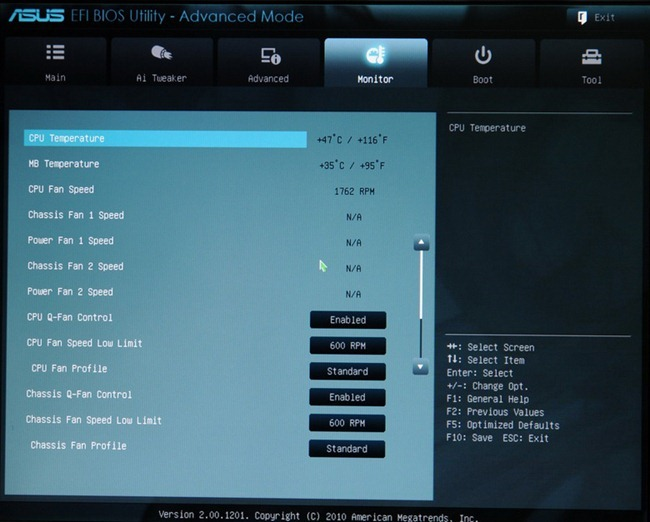
\includegraphics[width=\linewidth]{ASUS-EFI-screenshot}
\caption{So kann die UEFI Konfigurationsoberfläche aussehen$^{\decimal{footnote}}$}

\end{figure}
Um auch drahtlose Eingabegeräte zu unterstützen, haben viele UEFI Systeme einen ganzen Bluetooth-Stack an Board. Außerdem wird die Fähigkeit benötigt, hochqualitative Grafiken mit hoher Auflösung und Farbtiefe ausgeben zu können, was mit der Standardisierung des \textit{Graphics Output Protocol (GOP)} erreicht. Auch können Hersteller jetzt zum Erstellen von Konfigurationsoberflächen auf der \textit{Human Interface Infrastructure (HII)} aufbauen, die eine Art Toolkit bzw. Standardisierung von Bedienungselementen ist.

Auch auf der Netzwerkseite hat sich einiges getan: So gehört jetzt der \textit{PXE (Preboot eXecution Environment)} Standard zum Booten von Betriebssystemabbildern, die auf anderen Rechnern im Netzwerk gespeichert sind, zum Standard. Des weiteren bringt UEFI einen vollständigen eigenen TCP/IP Netzwerkstack mit, der auch parallel zu dem des Betriebssystems weiterlaufen kann, etwa als runtime service für Fernwartungszwecke.

UEFI bietet auch eine Shell, über die Befehle eingegeben werden oder Programme gestartet werden können. Diese ist aber nicht immer Teil des UEFI eines Systems, kann aber z.B. aus Intels TianoCore Projekt nachinstalliert werden.
\subsubsection{Secure Boot}
Die wohl kontroverseste Funktion des UEFI Standards ist \textbf{UEFI Secure Boot}. Diese Funktion erlaubt, dass nur kryptographisch signierte Bootloader und Betriebssysteme geladen werden können und soll so das Einnisten von Bootkits (Malware, von Bootsektor und Rootkit) verhindern, welche noch vor dem Betriebssystem starten und somit die Kontrolle über selbiges übernehmen kann.

Dieses Feature ist deshalb so kontrovers, da Microsoft als Vorraussetzung dafür, dass Computer sich mit dem Windows 8 Logo schmücken dürfen, festgelegt, dass dieses Feature standardmäßig aktiviert ist und sich Microsofts Schlüssel im System befinden muss.

Das hat den Effekt, dass letztendlich Microsoft bestimmen kann, welche Software auf den vom Endverbraucher gekauften Geräten laufen darf. Zwar ist dieses Feature wenigstens auf x86 Geräten abschaltbar, wodurch beliebige Betriebssysteme startfähig sind, allerdings ist der Großteil der Nutzer nicht in der Lage, sich durch Untermenüs in den Firmwareeinstellungen zu arbeiten oder weiß nicht einmal von dieser Einschränkung. Und auf ARM Geräten verbieten Microsofts Richtlinien sogar explizit die Möglichkeit des Abschaltens. Dadurch wird dem Nutzer endgültig die Kontrolle über das von ihm gekaufte Gerät genommen, da alternative Betriebssysteme somit auf die Gunst von Microsoft angewiesen sind. Diese bieten derzeit zwar einen Signierservice an, der für 99\$ eingesendete Binaries signiert und der von der Linux Distribution Fedora in Anspruch genommen wird, jedoch hat Microsoft jederzeit die Möglichkeit, Signaturen über Updates zurückzuziehen und es ist fraglich, wie lange dieser Signierungsservice bestehen bleibt.
\section{Fazit}
UEFI ist ein wichtiger Neuanfang, um das mittlerweile sehr veraltete BIOS und seine technischen Beschränkungen abzulösen. Sein modularer Aufbau und die Standardisierung über ein unternehmenübergreifendes Komitee gewährleisten Zukunftssicherheit und lassen auf einheitliche Funktionsweise hoffen.

Jedoch ist UEFI auch eine sehr komplexe Software und schon fast ein Betriebssystem. Damit stellt sich die Frage, warum 2 hochkomplexe Systeme gleichzeitig auf einem System laufen müssen und auch für beide Systeme Treiber bereitgestellt werden müssen, da Betriebssysteme in den meisten Fällen immer noch auf eigene Treiber angewiesen sind. Durch seine Komplexität ist UEFI auch ein potentielles Sicherheitsrisiko, da es etwa über den parallel weiterlaufenden Netzwerkstack kompromittiert und gesteuert werden kann und somit unterhalb des Betriebssystems das gesamte System steuern und manipulieren kann. Diese Manipulation kann nicht nur durch Malware, sondern auch durch scheinbar legitimere Module für \textit{DRM (Digital Rights Management, also Kopierschutz)} durchgeführt werden, die jeglichen Datenverkehr des Computers auf angebliche Urheberrechtsverletzungen scannen. Dies, aber auch das Ausnutzen von Sicherheitslücken ist so gut möglich, da zwar die Referenzimplementierung von UEFI unter einer BSD Lizenz steht, Änderungen aber nicht veröffentlicht werden müssen und UEFI immer noch auf proprietären Initialisierungscode aufsetzt, wodurch nur der Hardwarehersteller weiß, wie die Firmware funktioniert und was genau sie alles tut. Und auch Secure Boot kann ein gutes Mittel gegen Bootkits sein, solange aber Unternehmen wie Microsoft und nicht die Nutzer die Schlüsselgewalt über das system haben, leidet nur die Freiheit des Nutzers.

Insgesamt hat UEFI einige drängenden Probleme gelöst, andere (z.B. die Treiberproblematik) weitestgehend ignoriert und wiederum neue Probleme aufgeworfen.

\onecolumn
\section{Quellen}
\url{https://wiki.archlinux.org/index.php/UEFI}\\
\url{https://de.wikipedia.org/wiki/IBM-PC-kompatibler_Computer}\\
\url{https://en.wikipedia.org/wiki/Unified_Extensible_Firmware_Interface}\\
\url{https://en.wikipedia.org/wiki/BIOS}\\
\url{http://www.tomshardware.com/reviews/intel-uefi-firmware,2486.html}\\
\url{http://www.extremetech.com/computing/96985-demystifying-uefi-the-long-overdue-bios-replacement}\\
\url{http://www.howtogeek.com/56958/htg-explains-how-uefi-will-replace-the-bios/}\\
\url{http://faif.us/cast/2012/sep/27/0x32/}\\


\begin{figure}[h]
\begin{center}
\href{http://creativecommons.org/licenses/by-sa/3.0/de/}{
\includegraphics{cc-by-sa.png}}\\
Dieses Werk bzw. Inhalt ist lizenziert unter einer \href{http://creativecommons.org/licenses/by-sa/3.0/de/}{Creative Commons Namensnennung - Weitergabe unter gleichen Bedingungen 3.0 Deutschland Lizenz.}
\end{center}
\end{figure}
\end{document}
